\begin{figure}
\begin{center}
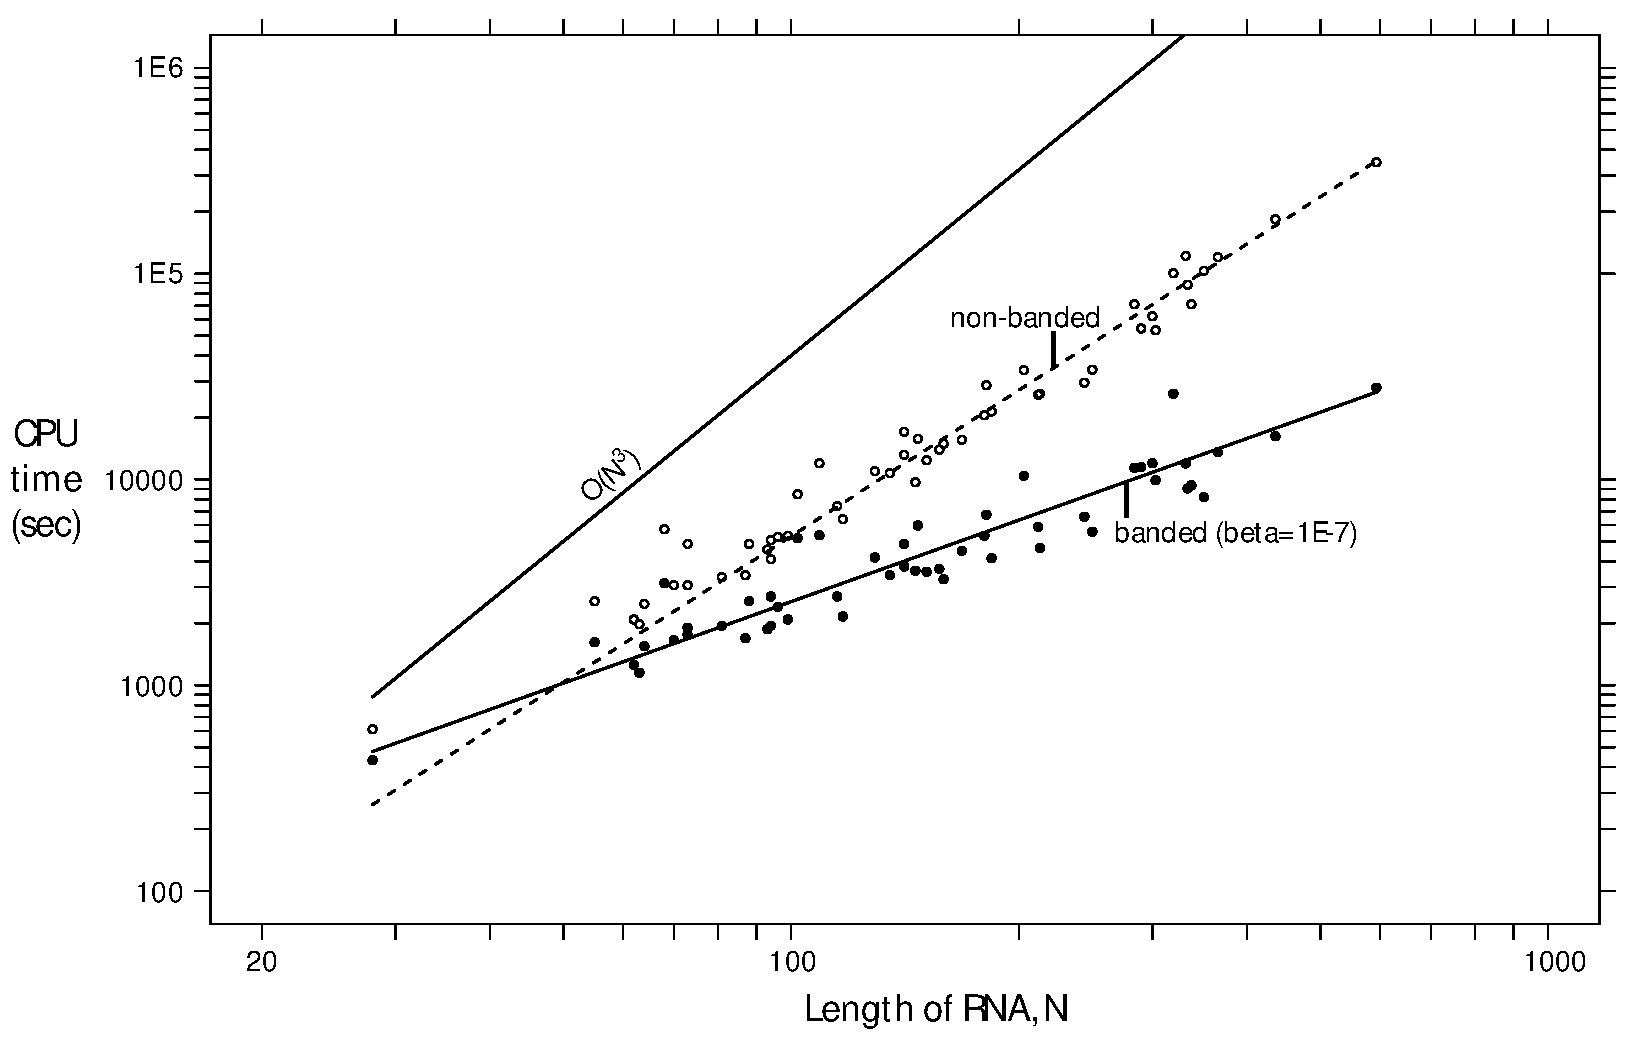
\includegraphics[width=6.4in]{figs/speedup_fit}
\caption{\textbf{CPU time required by CM searches with and without
    QDB.} The time required for searching the 1 Mb target pseudogenome
    with each of the 51 benchmark models is shown as a point, plotted
    on a log-log graph as a function of the average length of the RNA
    sequences in the query alignment; open circles are without QDB,
    and filled circles are with QDB (with the default $\beta =
    1e-7$). Lines represent fits to a power law ($aN^b$), showing that
    for a fixed $L=$ 1 Mb target database size, the standard CYK
    algorithm empirically scales as $N^{XXX}$ and the QDB algorithm
    scales as $N^{XXX}$. A line showing the worst-case upper bound of
    $O(N^3)$ is shown for comparison. }
\label{fig:speedup}
\end{center}
\end{figure}
